% \documentclass{report}

% \usepackage{subcaption} % package for subfigures
% \usepackage{hyperref}  % package for linking figures etc
% \usepackage{enumitem}  % package for description with bullets
% \usepackage{graphicx}  % package for importing images
% \usepackage{mathtools} % package for math equation
% \usepackage{mathrsfs}  % package for math font
% \usepackage{indentfirst} % package for getting ident after section or paragraph
% \usepackage[export]{adjustbox}
% \usepackage{multirow}  % package for tables, multir
% \usepackage{amssymb}
% % \usepackage{tabu}   % for tables 
% \setlength{\parindent}{2em} % how much indent to use when we start a paragraph

% \graphicspath{ {./theory/figures/} }       % path for images

% \begin{document}

\chapter{Tube Proposal Network}

One of the basic elements of ActionNet is \textbf{Tube Proposal Network}(TPN). The main purpose of this network is to propose
\textbf{Tube of Interest}(TOIs). These tubes are likely to contain an known action and are consisted of some 2D boxes
(1 for each frame). TPN is inspired from RPN introduced by FasterRCNN (\cite{Ren:2015:FRT:2969239.2969250}), but instead of images, TPN
is used in videos as show in \cite{DBLP:journals/corr/HouCS17}. In full correspondence with RPN, the structure
of TPN is similar to RPN. The only difference, is that TPN uses 3D Convolutional Layers and 3D anchors instead of 2D. \par
We designed 2 main structures for TPN. Each approach has a different definition of the used 3D anchors.
The rest structure of the TPN is mainly the same with some little differences in the regression layer. \par
Before describing TPN, we present the preprocess procedure which is the same for both approaches.

\section{Preparation for TPN}

\subsection{Preparing data}

Our architecture gets as input a sequnece of frames which has a fixed size in widht, height and duration. However, each video has different resolution. That's creates the
need to resize each frame before. As mentioned in previous chapter, the first element of our network is a 3D RenNet taken from \cite{hara3dcnns}. This network is designed to
get images with dimensions (112,112). As a result, we resize each frame from datasets' videos into (112,112) frames. In order to keep aspect ratio, we pad each frame either
left and right, either above and bellow depending which dimension is bigger. In figure  \ref{fig:Preprocess_example} we can see the original frame and the resize and padded one.
In full correspondance, we resize the groundtruth bounding boxes for each frame (figure \ref{fig:original_image_rois} and \ref{fig:trans_image_rois} show that).

\begin{figure}[h]
  \centering
  \begin{subfigure}{0.35\textwidth}
    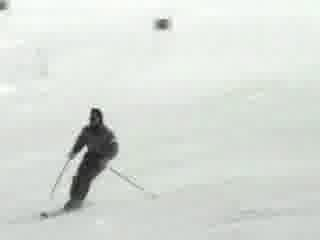
\includegraphics[width=\textwidth]{./figures/original_image.jpg}
    \caption{}
    \label{fig:original_image}
  \end{subfigure}
  \hfill
  \begin{subfigure}{0.35\textwidth}
    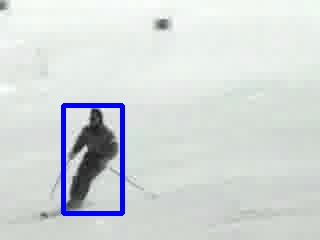
\includegraphics[width=\textwidth]{./figures/original_image_rois.jpg}
    \caption{}
    \label{fig:original_image_rois}
  \end{subfigure}
  \hfill
  \begin{subfigure}{0.35\textwidth}
    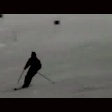
\includegraphics[width=\textwidth]{./figures/transformed_image.jpg}
    \caption{}
    \label{fig:trans_image}
  \end{subfigure}
  \hfill
  \begin{subfigure}{0.35\textwidth}
    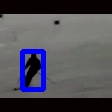
\includegraphics[width=\textwidth]{./figures/transformed_image_rois.jpg}
    \caption{}
    \label{fig:trans_image_rois}
  \end{subfigure}

  \caption{ At (a), (b) frame is its original size and at (c), (d) same frame after preprocessing part}
  \label{fig:Preprocess_example}
\end{figure}


\subsection{3D ResNet}
Before using Tube Proposal Network, we spatio-temporal features from the video. In order to do so, we extract the 3 first Layers of a
pretrained 3D ResNet. It is pretrained in Kinetics dataset \cite{DBLP:journals/corr/KayCSZHVVGBNSZ17} for sample duration = 16 and
sample size = (112,122). \par
This network normally is used for classifying the whole video, so some of its layers use temporal stride = 2.
We set their temporal stride equal to 1 because we don't want to miss any temporal information during the process.
So, the output of the third layer is a feature maps with dimesions (256,16,7,7). We feed this feature map to TPN, which is described
in following sections.

\section{ 3D anchors as 6-dim vector}
\subsection{First Description}
We started desinging our TPN inspired by \cite{DBLP:journals/corr/HouCS17}. We consider each anchor as a 3D bounding box written as
$(x_1, y_1, t_1, x_2, y_2, t_2)$ where $x_1, y_1, t_1$
are the upper front left coordinates of the 3D and $x_2, y_2, t_2$ are the lower back left as shown in figure \ref{fig:anchor_6d}.
\begin{figure}[h]
  \centering
  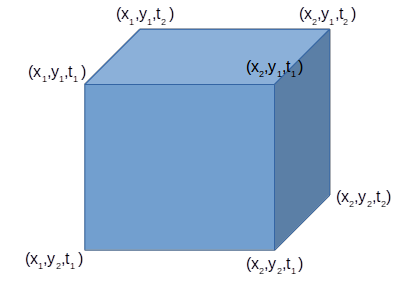
\includegraphics[scale=0.5]{anchor_6d}
  \caption{An example of the anchor $(x_1,y_1,t_1,x_2,y_2,t_2)$}
  \label{fig:anchor_6d}
\end{figure}

The main advantage of this approach is that except from x-y dims, dimension of time is mutable. As a result, the proposed TOIs have
no fixed time duration. This will help us deal with untrimmed videos, because proposed TOIs would exclude background frames.
For this approach, we use \textbf{n=4k=60} anchors for each pixel in the feature map of TPN. We have k anchors for each sample
duration( 5 scales of 1, 2, 4, 8, 16, 3 aspect ratios of 1:1, 1:2, 2:1 and 4 durations of 16,12,8,4 frames).
In \cite{DBLP:journals/corr/HouCS17},  network's anchors are defined according to the dataset most common anchors. This, however,
creates the need to redesign the network for each dataset. In our approach, we use the same anchors for both datasets, because we want our network not
to be dataset-specific but to be able to generalize for several datasets. As sample duration, we chose 16 frames per video segment because
our pre-trained ResNet is trained for video clips with that duration.
So the structure of TPN is:
\begin{itemize}
\item 1 3D Convolutional Layer with kernel size = 3, stride = 3 and padding = 1
\item 1 classification layer outputs \textit{2n scores} whether there is an action or not for \textit{n tubes}.
\item 1 regression layer outputs \textit{6n coordinates} ($x_1,y_1,t_1,x_2,y_2,t_2$) for \textit{n tubes}.
\end{itemize}

which is shown in figure \ref{fig:tpn_1_1}
\begin{figure}[h]

  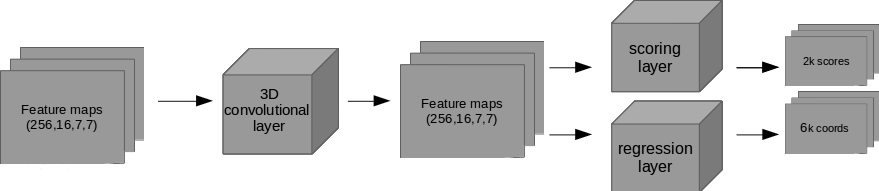
\includegraphics[width=1.\textwidth]{tpn_1_1}
  \caption{Structure of TPN}
  \label{fig:tpn_1_1}
\end{figure}

The output of TPN is the k-best scoring cuboid, in which it is likely to contain an action.
% \subsection{Preparing Data for training}


\subsection{Training}
As mentioned before, TPN extracts TOIs as 6-dim vectors. For that reason, we modify out groundtruth ROIs to groundtruth Tubes.
We take for granted that the actor cannot move a lot during 16 frames, so that's why we use this kind of tubes. As shown 
in figure \ref{fig:gt_tubes_and_rois}, these tubes are 3D boxes which include all the groundtruth rois, which are different
for each frame.

\begin{figure}[h]
  \centering
  \begin{subfigure}{0.15\textwidth}
    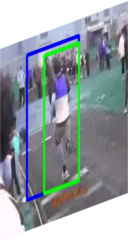
\includegraphics[width=\textwidth]{output/img_0.jpg}
  \end{subfigure}
  \begin{subfigure}{0.15\textwidth}
    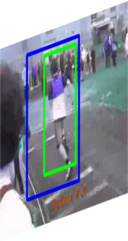
\includegraphics[width=\textwidth]{output/img_3.jpg}
  \end{subfigure}
  \begin{subfigure}{0.15\textwidth}
    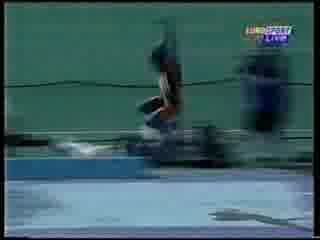
\includegraphics[width=\textwidth]{output/img_5.jpg}
  \end{subfigure}
  \begin{subfigure}{0.15\textwidth}
    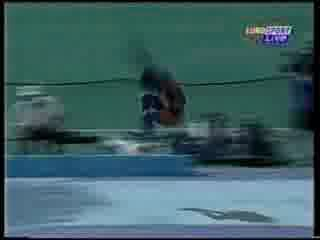
\includegraphics[width=\textwidth]{output/img_7.jpg}
  \end{subfigure}
  \begin{subfigure}{0.15\textwidth}
    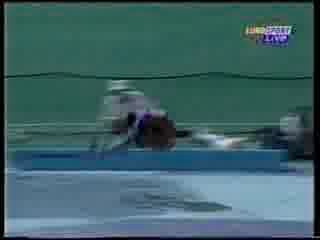
\includegraphics[width=\textwidth]{output/img_11.jpg}
  \end{subfigure}
  \begin{subfigure}{0.15\textwidth}
    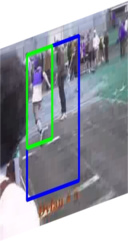
\includegraphics[width=\textwidth]{output/img_15.jpg}
  \end{subfigure}
  \caption{Groundtruth tube is coloured with blue and groundtruth rois with colour green}
  \label{fig:gt_tubes_and_rois}
\end{figure}

For training procedure, for each video, we randomly select a part of it which has duration 16 frames. We consider an anchor as foreground if its overlap score with a groundtruth
action tube is bigger than 0.5. Otherwise, it is considered as background anchor. We use scoring layer in order to correctly classify those anchors and we use
Cronss Entropy Loss as loss function. We have a lot of anchors for proposing an anction but few numbers of actions, so we choose 256 anchors in total for each batch. We set the maximum
number of foreground anchors to be  25\% of the 256 anchors and the rest are the background.\par
Classifying correctly an anchor isn't enough for proposing an action tube. It is necessary to overlap as much as possible with the groundtruth action tubes. That's the reason we use a
regression layer. This layer ``moves'' the cuboid closer to the area that it is believed that is closer to the action.
For regression loss we use smooth-L1 loss as proposed in \cite{DBLP:journals/corr/GirshickDDM13}. In order to calculate
the regression targets, we use pytorch FasterRCNN implementation (\cite{jjfaster2rcnn}) for bounding box regression and 
we modified the code in order to extend it for 3 dimensions. % \textbf{TODO more details}
So we have:
\[ \begin{matrix}
    t_x = (x-x_a)/w_a, & t_y = (y-y_a)/h_a, & t_z= (z-z_a)/d_a, \\
    t_w= log(w/w_a), & t_h= log(h/h_a), & t_d = log(d/d_a), \\
    t^*_x = (x^* - x_a)/w_a, & t^*_y = (y^* - y_a)/h_a, & t^*_z = (z^* - z_a)/d_a, \\
    t^*_w = log(w^* /w_a), & t^*_h = log(h^*/h_a), & t^*_d = log(d^*/d_a),
    % t∗x= (x∗−xa)/wa,  t∗y= (y∗−ya)/ha,t∗w= log(w∗/wa),  t∗h= log(h∗/ha)
  \end{matrix}
\]
where \textit{x, y, z, w, h, d} denote the 3D box's center coordinates and its width, height and duration. Variables $x, x_a, \text{ and } x^*$
are for the predicted box, anchor box, and groundthruth box respectively (likewise for \textit{y, z, w, h, d}). Of course, we calculate the
regression loss only for the foreground anchors and not for the background, so at the most we will calculate 64 targets
for each batch. \par

To sum up training procedure, we train 2 layers for our TPN, scoring and reggression layers. The training loss includes the training losses
obtained by these layers and its formula is:
% \[ L  = \frac{1}{N_{cls}} \sum_iL_{cls}(p_i, p^*) + \frac{1}{N_{reg}}\sum_ip_i^*L_{reg}(t_i,t_i^*) \]
\[ L  =  \sum_iL_{cls}(p_i, p_i^*) + \sum_ip_i^*L_{reg}(t_i,t_i^*) \]
where:
\begin{itemize}
\item $L_{cls} $ is the Cross Entropy loss we use for classifying the anchors, with $p_i$ is the predicted label, $p_i^*$ is the groundtruth class and
  $p_i, p_i^* \in \{0,1\}$
\item $L_{reg} $ is the smooth-L1 loss function, which multiply it with $p_i^*$ in order to set active only when we have a positive anchor $(p_i^* = 1)$
  and to be deactivated for background anchors $(p_i^* = 0)$.
\end{itemize}

\subsection{Validation}

Validation procedure is a bit similar to training procedure.
We randomly select 16 frames from a validation video and we examine if there is at least 1 proposed TOI
which overlaps $\ge$ 0.5 with each groundtruth action tube and we get recall score. 
In order to get good proposals, after getting classification scores and targets prediction from the
corresponding layers, we use Non-Maximum Suppresion (NMS) algorithm.  We set NMS threshold equal with 0.7,
and we keep the first 150 cuboids with the biggest score.

\subsection{Modified Intersection over Union(mIoU) TODO check again} 
During training, we get numerous anchors. We have to classify them as foreground anchors or
background anchors. Foreground anchors are those which contain some action, and, respectively, background
don't. As presented before, IoU for cuboids calculates the ratio between volume of overlap and volume of
union.
Intuitively, this criterion is good for evaluating 2 tubes if they overlap but it has one big drawback:
it considers x-y dimesions to have same importance with time dimension, which we do not desire. That's becase
firstly we care to be accurate in time dimension, and then we can fix x-y domain.
As a result, we change the way we calculate the Intesection Over Union. We calculate seperately
the IoU in x-y domain (IoU-xy) and in t-domain (IoU-t). Finally, we multiply them in order to get the final IoU.
So the formula for 2 tubes ($x_1, y_1, t_1, x_2, y_2, t_2$) and ($x'_1, y'_1, t'_1, x'_2, y'_2, t'_2$) is:
\[ IoU_{xy} = \frac{ \text{Area of Overlap in x-y}} { \text{Area of Union in x-y}}  \]
\[ IoU_t = \frac { max(t_1, t'_1) - min(t_2, t'_2)} {min(t_1,t'_1) - max(t_2,t'_2)} \]
\[ IoU = IoU_{xy} \cdot  IoU_t \]
The above criterion help us balance the impact of time domain in IoU. For example, let us consider 2 anchors:
a = (22, 41, 1, 34, 70, 5) and b = (20, 45, 2, 32, 72, 5). These 2 anchors in x-y domain have IoU score equal to 0.61.
But they are not exactly overlaped in time dim. Using the first approach we get 0.5057 IoU score and using the
second approach we get 0.4889. So, the second criterion would reject this anchor, because there is a difference in time
duration.  \par

In order to verify our idea, we train TPN using both IoU and mIoU criterion for tube-overlapping. At Table \ref{table:iou_miou}
we can see the performance in each case for both datasets, JHMDB and UCF. Recall threshold for this case is 0.5 and during validation,
we use regular IoU for defining if 2 tubes overlap.
\begin{table}[h]
\centering
  \begin{tabular}{|| c | c || c ||}
    \hline
    \textbf{Dataset} & \textbf{Criterion} & \textbf{Recall(0.5)} \\
    \hline  \hline
    \multirow{2}{4em}{JHMDB} & IoU & 0.70525 \\
    \cline{2-3}
    {} & mIoU & 0.7052 \\
    \hline
    \multirow{2}{4em}{UCF} & IoU & 0.4665 \\
    \cline{2-3}
    {} & mIoU & 0.4829 \\
    \hline      
  \end{tabular}
  \caption{Recall results for both datasets using IoU and mIoU metrics}
  \label{table:iou_miou}
\end{table}

Table \ref{table:iou_miou} shows that modified-IoU give us slightly better recall performance only in UCF dataset. Thats reasonable, because JHMDB dataset
uses trimmed videos so time duration doesn't affect a lot. So, from now own, during training we use mIoU as overlapping scoring policy.

\subsection{Improving TPN score}
After first test, we came with the idea that in a video lasting 16 frames, in time domain, all kind of actions can be seperated in the following categories:
\begin{enumerate}
\item Action starts in the n-th  frame and finishes after the 16th frame of the sampled video.
\item Action has already begun before the 1st frame of the video and ends in the n-th frame.
\item Action has already begun before the 1st frame of the video and finishes after the 16th video frame.
\item Action starts and ends in that 16 frames of the video.
\end{enumerate}

On top of that, we noticed that most of actions, in our datasets, last more that 16 frame. So, we came with the idea to add  1 scoring layer and 1 reggression layer
which will proposed ToIs with fixed duration equal with sample duration and they will take into account the spatial information produced by activation maps.
The new structure of TPN is shown in figure \ref{fig:tpn_1_2}. After getting proposals from both scores, we concat them with ration 1:1 between ToI extracted
from those 2 subnetworks.

\begin{figure}[h]
  \centering
  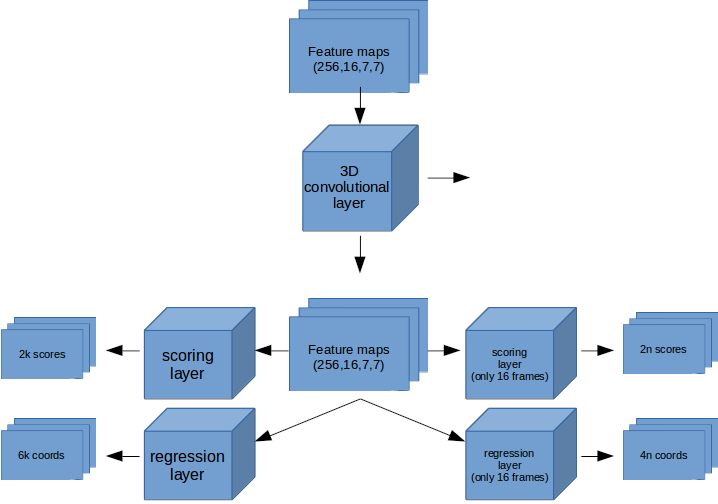
\includegraphics[scale=0.5]{tpn_1_2}
  \caption{TPN structure after adding 2 new layers, where k = 5n.}
  \label{fig:tpn_1_2}
\end{figure}
Our goal is to ``compress'' feauture maps in temporal dimension in order to propose action tubes  according only to the spatial information.
So, we came with 2 techniques for doing such thing:
\begin{enumerate}
\item Use 3D Convolutional Layers with kernel size = (sample duration, 1,1), stride =1 and no padding for scoring and regression.
  This kernel ``looks'' only in the temporal dimension of the activation maps and doesn't consider any spatial dependencies.
\item Get the average values from temporal dimension and then use a 2D Convolutional Layer for scoring and regression.
\end{enumerate}

% \textbf{TODO na perigrapsw oti thelw na exw ola ta xronika features}
\par
Training and Validation procedures remain the same. The only big difference is that now we have from 2 difference system proposed TOIs. So, we first concate
them and, then, we follow the same procedure. For training loss, we have 2 different cross-entropy losses and 2 different smooth-L1 losses, each for every
layer correspondly. So training loss is, now, defined as :

  % \begin{aligned}
 % L  =  \sum_iL_{cls}(p_i, p_i^*) + \sum_iL_{cls}(p_{fixed,i}, p_{fixed,i}^*) +  
 %  \sum_ip_i^*L_{reg}(t_i,t_i^*) + \sum_ip_{fixed,i}^*L_{reg}(t_{fixed,i},t_{fixed,i}^*) 
% L  =2


% \[ L  =  \sum_iL_{cls}(p_i, p_i^*) + \sum_iL_{cls}(p_{fixed,i}, p_{fixed,i}^*) +  \newline
%   \sum_ip_i^*L_{reg}(t_i,t_i^*) + \sum_ip_{fixed,i}^*L_{reg}(t_{fixed,i},t_{fixed,i}^*) \]
% \end{aligned}


\begin{equation} 
\begin{split}
 L  =  \sum_iL_{cls}(p_i, p_i^*) + \sum_iL_{cls}(p_{fixed,i}, p_{fixed,i}^*) + \\
   \sum_ip_i^*L_{reg}(t_i,t_i^*) + \sum_ip_{fixed,i}^*L_{reg}(t_{fixed,i},t_{fixed,i}^*) 
  % \sum_iL_{cls}(p_i, p_i^*) + \sum_iL_{cls}(p_{fixed,i}, p_{fixed,i}^*) 
\end{split}
\end{equation}

where:
\begin{itemize}
  \item $L_{cls} $ is the Cross Entropy loss we use for classifying the anchors, with $p_i$ is the predicted label, $p_i^*$ is the groundtruth class and
  $p_i, p_i^* \in \{0,1\}$
\item $L_{reg} $ is the smooth-L1 loss function, which multiply it with $p_i^*$ in order to set active only when we have a positive anchor $(p_i^* = 1)$
  and to be deactivated for background anchors $(p_i^* = 0)$.
\item $p_i $ are the anchors from scoring layers with mutable time duration and $p_i^*$ are their corresponding groundtruth label.
\item $p_{fixed,i} $ are the anchors from scoring layers fixed time duration = 16 and $p_{fixed,i}^*$ are their corresponding groundtruth label.
\end{itemize}

We train our TPN Network using both techniques and their recall performance is show in Table \ref{table:add_16}.

\begin{table}[h]
  \centering
  \begin{tabular}{||c | c | c || c ||}
    \hline
    \textbf{Dataset} & \textbf{Fix-time anchors} & \textbf{Type} & \textbf{Recall(0.5)} \\
    \hline  \hline
    \multirow{3}{4em}{JHMDB} & No &  - & 0.7052 \\
    \cline{2-4}
    {} & \multirow{2}{*}{Yes} & Kernel & 0.6978 \\
    \cline{3-4}
    {} & {} & Mean & 0.7463 \\
    \hline
    \multirow{3}{4em}{UCF} & No & - & 0.4829 \\
    \cline{2-4}
    {} & \multirow{2}{*}{Yes} & Kernel & 0.4716 \\
    \cline{3-4}
    {} & {} & Mean & 0.4885 \\
    \hline      
  \end{tabular}
  \caption{Recall results after adding fixed time duration anchors}
  \label{table:add_16}
\end{table}

As we can see from the previous results, the new layers increased recall performance significantly. On top of that, Table \ref{table:add_16} shows that
getting the average values from time dimension gives us the best results.


\subsection{Adding regressor}
The output of TPN is the $\alpha$-highest scoring anchors moved according to their regression prediction. After that, we have to translate the anchor into tubes.
In order to do so, we add a regressor system which gets as input TOIs' feature maps and returns a sequence of 2D boxes, each for every frame.
The only problem is that the regressor needs a fixed input size of featuremaps. This problem is already solven by R-CNNs which use roi pooling and roi align
in order to get fixed size feature maps from ROIs with changing sizes. In our situation, we extend roi align operation, presented by Mask R-CNN, and we
call it \textbf{3D Roi Align}.

\paragraph{3D Roi Align}
3D Roi align is a modification of roi align presented by Mask R-CNN (\cite{DBLP:journals/corr/HeGDG17}). The main difference between those two is that Mask R-CNN's roi align uses
bilinear interpolation for extracting ROI's features and ours 3D roi align uses trilinear interpolation for the same reason. Again, the 3rd dimension is
time.
So, we have as input a feature map extracted from ResNet34 with dimensions (64,16,28,28) and a tensor containing the proposed TOIs.
For each TOI whose actiovation map whose size is (64,16,7,7), we get as output a feature map with size (64, 16, 7, 7). \par

\subsubsection{Regression procedure}
At first, for each proposed ToI, we get its corresponding activation maps using 3D Roi Align. These features are given as input to a regressor. This regressor returns 16 $\cdot$ 4 predicted
transforms $(\delta_x,\delta_y, \delta_w,\delta_h)$, 4 for each frame, where $ \delta_x, \delta_y$ specify the coordinates of proposal's center and $\delta_w, \delta_h$ its width and height, as specified
in \cite{DBLP:journals/corr/GirshickDDM13}.  We keep only the predicted translations, for the frames that are $\ge t_1$ and $< t_2$ and for the other frames, we set a zero-ed 2D box. 
After that, we modify each anchor from a cuboid written like $(x_1,y_1,t_1, x_2, y_2, t_2)$ to a sequence of 2D boxes, like: \\
$(0,0,0,0, ..., x_{T_1},y_{T_1},x'_{T_1},y'_{T_1}, ... ,x_{i},y_{i},x'_{i}, ..., x_{T_2},y_{T_2},x'_{T_2},y'_{T_2}, 0,0,0,0, ....)$, where
\begin{itemize}
\item $ T_1 \le i \le T_2$, for $T_1 < t_1 + 1,  T_2 < t_2 \text{ and }T_1,T_2 \in \mathbb{Z} $
\item $ x_i = x_1, y_i= y_1, x'_i = x_2, y'_i = y_2 $.
\end{itemize}

\paragraph{ Training}
In order to train our Regressor, we follow about the same steps followed previously for previous TPN's training procedure. This means that
we randomly pick 16 ToI from those proposed by TPN's scoring layer. From those 16 tubes, 4 are foreground tubes, which meands 25\% of the total
number of the tubes as happened previously. We extract their corresponding features using 3D Roi Algin and calculate their targets like
we did for regression layer. We feed Regressor Network with these features and compare the predicted targets with the expected.
Again, we use smooth-L1 loss for loss function, calculated only for foreground ToIs. So, we add another parameter in
training loss formula which is now defines as:
% \textbf{TODO Describe training procedure}
% \textbf{TODO Training Loss formula}
\begin{equation} 
\begin{split}
 L  =  \sum_iL_{cls}(p_i, p_i^*) + \sum_iL_{cls}(p_{fixed,i}, p_{fixed,i}^*) + \\
 \sum_ip_i^*L_{reg}(t_i,t_i^*) + \sum_ip_{fixed,i}^*L_{reg}(t_{fixed,i},t_{fixed,i}^*) + \\
  \sum_iq_i^*L_{reg}(c_{i}, c_{i}^*) + \\
  % \sum_iL_{cls}(p_i, p_i^*) + \sum_iL_{cls}(p_{fixed,i}, p_{fixed,i}^*) 
\end{split}
\end{equation}
where  except the previously defined parameters, we set  $c_{i} $ as the regression targets for picked tubes $q_i$.
These tubes are the ones randomly selected from the proposed ToIs and $q_i^*$ are their corresponding groundtruth action tubes, which are the closest to each $q_i$ tube.
Again we use $q_i^*$ as a factor because we consider a tube as background when it doesn't overlaps with any groundtruth action tube more that 0.5 .

\subsubsection{First regression Network} \textbf{Na pw gia to normalize kai to pooling kernel}\par
The architecture of reggression network is show in Figure \ref{fig:regressor_3d}, and it is described below:
\begin{figure}[h]
  \centering
  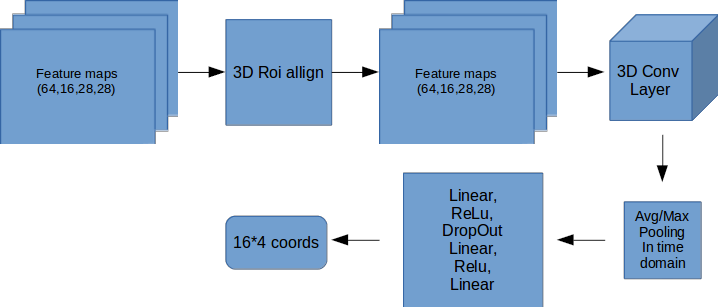
\includegraphics[scale=0.48]{regressor_1_1}
  \caption{Structure of Regressor}
  \label{fig:regressor_3d}
\end{figure}

\begin{enumerate}
\item Regressor is consisted, at first, with a 3D convolutional layer with kernel = 1, stride = 1 and no padding. This layer gets as input ToI's normalized activation map extracted by 3D Roi Align.
\item After that, we calculate the average value in time domain, so from a feature map with dimensions (64,16,7,7), we get as output a feature map (64,7,7).
\item These feature maps are given as input to a Linear layer followerd by a Relu Layer, a Dropout Layer, another Linear Layer and Relu Layer and a final Linear.
\end{enumerate}

% \textbf{NA DW TA FEATURE MAPS POIA XRISIMOPOIISA}
\begin{table}[h]
  \centering
  \begin{tabular} {||c | c || c  c  c ||}
    \hline
    \textbf{Dataset} & \textbf{Pooling} & Cuboid Recall & Single Rois Recall & Single rois follow up\\
    \hline                
    \multirow{2}{*}{JHMDB} & avg & 0.8545 & 0.7649 & 0.7183 \\
    \cline{2-5}
    {} & max & 0.8396 & 0.7761 & 0.5783 \\
    \cline{1-5}
    \multirow{2}{*}{UCF} & avg & 0.5319 & 0.4694 & 0.5754 \\
    \cline{2-5}
    {} & max & 0.5190 & 0.5021 & 0.5972 \\
    \cline{1-5}
                                   
  \end{tabular}
  \caption{Recall results after convertying cuboids into sequences of frames}
  \label{table:reg_1_1}
\end{table}

\textbf{TODO Comment results - Tommorow - write about reduction from tubes to rois}
As the above results show, when we translate a TOI into a sequence of ROIs, recall reduces about 20-30\%, which is a big problem. 

\subsection{Changing Regressor - from 3D to 2d}
After getting first recall results, we experiment using another architecture for the regressor network. Instead of having a 3D Convolutional
Layer, we will use a 2D Convolutional Layer in order to treat the whole time dimension as one during convolution operation. So, as shown in Figure \ref{fig:reg_1_2},
the $2^{nd}$ Regression Network is about the same with first one, with 2 big differences:
\begin{enumerate}
\item We performing a pooling operation at the feature maps extracted by 3D Roi Align operation
\item Instead of a 3D Convolutional Layer, we have a 2D Convolutional Layer with kernel size = 1, stride = 1 and no padding.
\end{enumerate}

\begin{figure}[h]

  \centering
  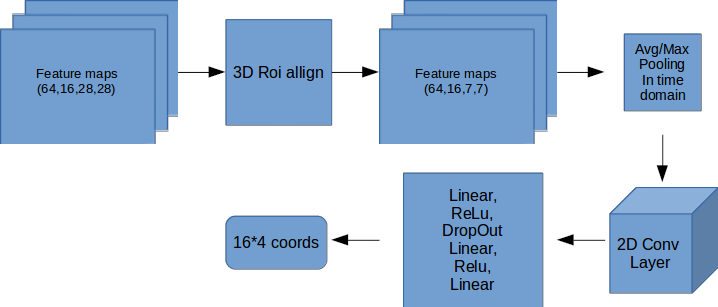
\includegraphics[scale=0.48]{regressor_1_2}
  \caption{Structure of Regressor}
  \label{fig:reg_1_2}
\end{figure}

On top of that, we tried to determine which feature map is the most suitable  for getting best-scorig recall performance. This feature map will be given as
input to Roi Algin operation.  At Table \ref{table:reg_1_2}, we can see the recall performance for different feature maps and different pooling methods.
\\
\textbf{Pending explain SR, SRF}

\begin{table}[h]
  \centering
  \begin{tabular}{||c | c | c || c  c  c ||}
    \hline
    \textbf{Dataset} & \textbf{Pooling} & \textbf{F. Map} & \textbf{Recall} &  \textbf{ Recall SR}  &  \textbf{Recall SRF)} \\
    \hline
    \multirow{6}{*}{JHMDB} & \multirow{3}{*}{mean} & 64 &  0.6828  & 0.5112  & 0.7610 \\
    \cline{3-6}
    {} & {} & 128 & 0.8694 & 0.7799 & 0.6756 \\
    \cline{3-6}
    {} & {} & 256 & 0.8396 & 0.7687 & 0.7029 \\
    \cline{2-6}
    {} & \multirow{3}{*}{max} & 64 &  0.8582 & 0.7985 & 0.5914\\
    \cline{3-6}
    {} & {} & 128 & 0.8358 & 0.7724 & 0.8118 \\
    \cline{3-6}
    {} & {} & 256 & 0.8657 & 0.8022 & 0.7996 \\
    \hline
    \multirow{6}{*}{UCF} & \multirow{3}{*}{mean} & 64 & 0.5055 & 0.4286 & 0.5889 \\
    \cline{3-6}
    {} & {} & 128 & 0.5335 & 0.4894 & 0.5893 \\
    \cline{3-6}
    {} & {} & 256 & 0.5304 & 0.4990 & 0.6012 \\
    \cline{2-6}
    {} & \multirow{3}{*}{max} & 64 & 0.5186 & 0.4990 & 0.5708 \\
    \cline{3-6}
    {} & {} & 128 & 0.5260 & 0.4693 & 0.5513 \\
    \cline{3-6}
    {} & {} & 256 & 0.5176 & 0.4878 & 0.6399 \\
    \hline


  \end{tabular}
  \caption{}
  \label{table:reg_1_2}
\end{table}

\textbf{Pending... commentary}
As we noticed from the above results, our system has difficulty in translating 3D boxes into 2D sequence of ROIs. So, that makes us rethink the way we designed
our TPN.


\section{ 3D anchors as 4k-dim vector}
In this approach, we set 3D anchors as 4k coordinates (k = 16 frames = sample duration). So a typical anchor is written as ($x_1, y_1, x'_1, y'_1, x_2, y_2, ...$)
where $x_1, y_1, x'_1, y'_1 $ are the coordinates for the 1st frame, $x_2, y_2, x'_2, y'_2$ are the coordinates for the 2nd frame etc, as presented in \cite{DBLP:journals/corr/abs-1712-09184}.
In figure \ref{fig:anchor_4k} we can an example of this type of anchor.

\begin{figure}[h]
  \centering
  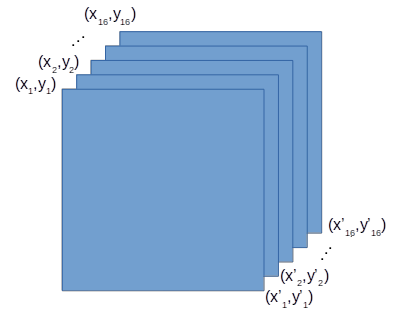
\includegraphics[scale=0.5]{anchor_4k}
  \caption{An example of the anchor $(x_1,y_1,x'_1,y'_1,x_2,y_2, ...)$}
  \label{fig:anchor_4k}
\end{figure}

The main advantage of this approach is that we don't need to translate the 3D anchors into 2D boxes, which caused many problems at the previous approach.
However, it has a big drawback, which is the fact that this type of anchors has fixed time duration.
In order to deal with this problem, we set anchors with different time durations, which are 16, 12, 8 and 4.
Anchors with duration $ < $ sample duration (16 frames) can be written as 4k vector with zeroed coordinateds in the frames bigger that the time duration. For example, an anchor with
2 frames duration, starting from the 2nd frame and ending at the 3rd can be written as (0, 0, 0, 0, $x_1, y_1, x'_1, y'_1, x_2, y_2, x'_2, y'_2$, 0, 0, 0, 0) if sample
duration is 4 frames. 

\begin{figure}[h]
  \centering
  % 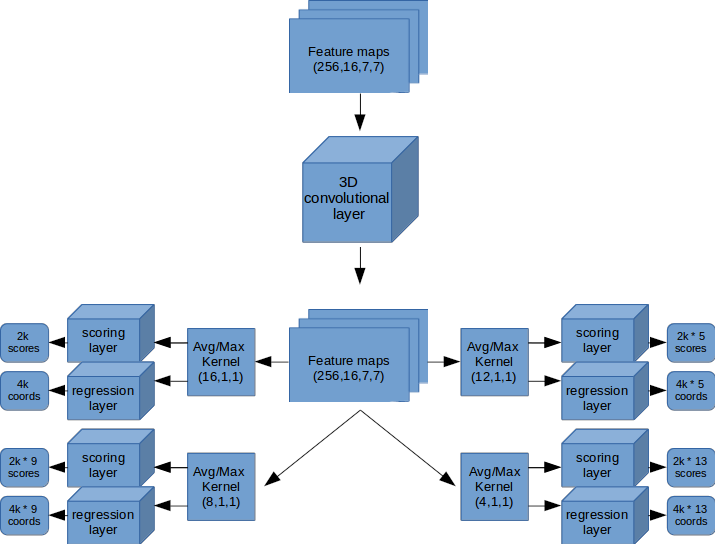
\includegraphics[width=1.\textwidth]{tpn_2}
  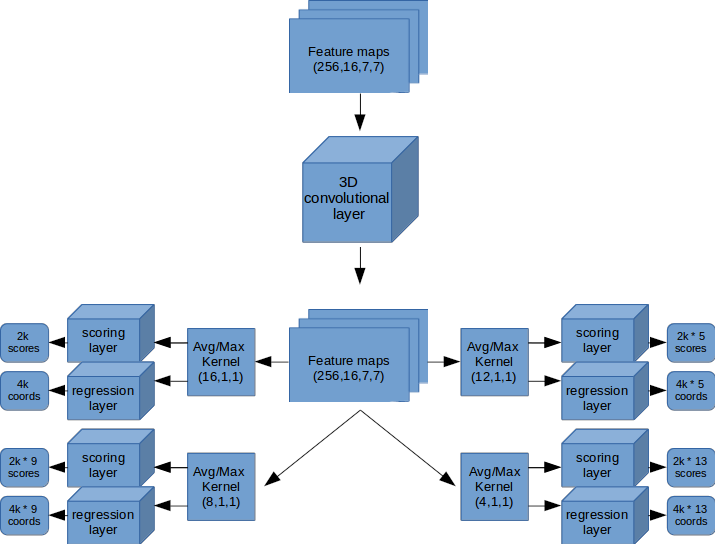
\includegraphics[scale=0.4]{tpn_2}
  \caption{The structure of TPN according to new approach}
  \label{fig:New_structure}
\end{figure}

This new approach led us to change the structure of TPN. The new one can is presented in figure \ref{fig:New_structure}. As we can see, we \
added scoring and regression layers for each duration. So, TPN follows the next step in order to propose action tubes:
\begin{enumerate}
\item At first, we get the feature map, extracted by ResNet, as input to a 3D Convolutional Layer with kernel size = 1, stride = 1 and no padding.
\item From Convolutional Layer, we get as output an activation map with dimensions (256,16,7,7). For reducing time dimension, we use 4 pooling layer,
  one for each sample duration with kernel sizes \textit{(16,1,1), (12,1,1,), (8,1,1) and (4,1,1)} and stride = 1,  for sample durations 16, 12, 8 and 4 respectively.
  So, we get activation maps with dimensions \textit{(256,1,7,7), (256,5,7,7), (256,9,7,7) and (256,13,7,7)}, in which

  \textbf{TODO na to teleiwsw...}
\item For ....
\end{enumerate}

\subsection{Training}
Training procedure stays almost the same like previous approach's. So, again, we randomly choose  a video segment and we consider anchors with overlap bigger than 0.8 with any groundtruth
tube, alongside with background anchors whose overlap is bigger that 0.1 and smaller than 0.3.

\begin{table}[h]
  \centering
  \begin{tabular}{||c | c || c  c c||}
    \hline
    \textbf{Dataset} & \textbf{Pooling} &  \textbf{Recall(0.5)} & \textbf{Recall(0.4)} & \textbf{Recall(0.3)} \\
    \hline  \hline
    \multirow{2}{4em}{JHMDB} & mean & 0.6866 & 0.7687 & 0.8582 \\
    \cline{2-5}
    {} & max &  0.8134 & 0.8694 & 0.9216 \\
    \hline
    \multirow{2}{4em}{UCF} & mean &  0.5435 & 0.6326 & 0.7075 \\
    \cline{2-5}
    {} & max & 0.6418 & 0.7255 & 0.7898 \\
    \hline
  \end{tabular}
  \caption{Recall results}
  \label{table:tpn_2_1}
\end{table}

\textbf{Pending... commentary + network structure}

\subsection{Adding regressor}
\textbf{Pending introduction...}
\textbf{Pending complete table...}
In full correspondance with the previous approach, we added an regressor for trying to find better results.
3D regressor

\begin{table}[h]
  \centering
  \begin{tabular}{||c | c || c  c  c||}
    \hline
    \textbf{Dataset} & \textbf{Feat. Map} & \textbf{Recall(0.5)} & \textbf{Recall(0.4)} & \textbf{Recall(0.3)}\\
    \hline
    \multirow{3}{*}{JHMDB} &  64 & Pending... \\
    \cline{2-5}
    {} & 128 & Pending... \\
    \cline{2-5}
    {} & 256 & Pending... \\
    \hline
    \multirow{3}{*}{UCF}  & 64 & Pending...\\
    \cline{2-5}
    {} & 128 & Pending...\\
    \cline{2-5}
    {} & 256 & Pending... \\
    \hline

  \end{tabular}
  \caption{}
  \label{table:reg_2_1}
\end{table}

\textbf{Pending commentary...}

\subsection{From 3D to 2D}
% \subsection{Changing Regressor - from 3D to 2d}
% After getting first recall results, we experiment using another architecture for the regressor network. Our idea was that we can treat feature maps like not having
% temporal dependencies between their frames. So, at first, we get from Roi Align operation activation maps with dimensions \textit{(k,64,16,7,7)} where k is the number
% of ToIs proposed for this video segment. We reshape this feature map to \textit{ (k*16,64,7,7) }, and in same time, we reshape their proposed action tubes from \textit{(k,16,4)}
% to \textit{(k*16,4)}. So, the new regression Network is consisted with:
% % \begin{enumerate}
% % \item a 2D Convolutional Network
% \paragraph{From 3D to 2d}
% The first idea we thought, was to change the first Convolutional layer from 3D to 2D. This means that we consider  features  not to have temporal dependencies for
% each frame. As we can see in the figure \ref{}, we got worse results, so, we rejected this idea.

% \subsection{Trying to  improve performance}
% TODO
% \subsection{Changing training procedure}
% TODO

\begin{table}[h]
  \centering
  \begin{tabular}{||c | c || c  c  c||}
    \hline
    \textbf{Dataset}  & \textbf{Feat. Map} & \textbf{Recall(0.5)} & \textbf{Recall(0.4)} & \textbf{Recall(0.3)}\\
    \hline
    \multirow{3}{*}{JHMDB} & 64 & 0.8358 & 0.9216 & 0.9739\\
    \cline{2-5}
    {} & 128 & 0.8172 & 0.9142 & 0.9627 \\
    \cline{2-5}
    {} & 256 & 0.7724 & 0.8731 & 0.9328 \\
    \hline
    \multirow{3}{*}{UCF} & 64 & 0.6368 & 0.7346 & 0.7737 \\ 
    \cline{2-5}
    {} & 128 & 0.6363 & 0.7133 & 0.7822 \\
    \cline{2-5}
    {} & 256 &  0.6363 & 0.7295 & 0.7822 \\
    \hline

  \end{tabular}
  \caption{}
  \label{table:reg_2_2}
\end{table}


\subsection{Changing sample duration}
\textbf{Pending commentary...}ψ
After trying all the previous version, we noticed that we get about the same recall performances. So, we thought that we could try
to reduce the sample duration. On top of that, we trained our network for sample duration = 8 and 4 frames.

\subsubsection{Without Regressor}

\begin{table}[h]
  \centering
  \begin{tabular}{|c | c || c c c|}
    \hline
    \textbf{Dataset} & \textbf{Sample dur} & \textbf{Recall(0.5)} &  \textbf{Recall(0.4)} &  \textbf{Recall(0.3)} \\
    \hline
    \multirow{2}{*}{JHMDB} & 8 & 0.9515 & 0.9888 & 1.0000 \\
    \cline{2-5}
    {} & 4 & 0.8843 & 0.9627 & 0.9888 \\
    \hline
    \multirow{2}{*}{UCF} & 8 & 0.7942 & 0.8877 & 0.9324\\
    \cline{2-5}
    {} & 4 & 0.7879 & 0.8924 & 0.9462 \\
    \hline
    
  \end{tabular}
  \caption{}
  \label{table:new_sample}
\end{table}

\subsubsection{with Regressor}                                             

\begin{table}[h]
  \centering
  \begin{tabular}{|c | c | c || c c c|}
    \hline
    \textbf{Dataset} & \textbf{Sample dur} & \textbf{Type} & \textbf{Recall(0.5)} &  \textbf{Recall(0.4)} &  \textbf{Recall(0.3)} \\
    \hline
    \multirow{4}{*}{UCF} & \multirow{2}{*}{8} & 2D & 0.8078 & 0.8870 & 0.9419 \\
    \cline{3-6}
    {} & {} & 3D & 0.8193 & 0.8930 & 0.9487 \\
    \cline{2-6}
    {} & \multirow{2}{*}{4}& 2D & 0.7785 & 0.8914 & 0.9457 \\
    \cline{3-6}
    {} & {} & 3D & Pending... \\
    \hline
    \multirow{4}{*}{JHDMBD} & \multirow{2}{*}{8} & 2D &  0.9366 & 0.9851 & 0.9925  \\
    \cline{3-6}
    {} & {} & 3D & Pending... \\
    \cline{2-6}
    {} & \multirow{2}{*}{4}& 2D & 0.9552 & 0.9963 & 1.0000 \\
    \cline{3-6}
    {} & {} & 3D & Pending... \\
    \hline
    
  \end{tabular}
  \caption{}
  \label{table:new_sample_reg}
\end{table}


% \end{document}

